\iffalse

Nico Casale
Cody Orazymbetov

ECE 592 Project 2

\fi

\documentclass[]{../ncmathy}

\begin{document}

To verify the time complexity for Dijkstra's algorithm empirically, we wrote a script to test a random collection of trips across NC. Since the running time is dependent on the number of nodes traversed, we decreased our threshold to 20 miles. This encourages the algorithm to use a larger number of hops in the paths it develops. Empirically, the plot below shows that the maximum number of hops required for most trips in NC, using 20 mile hops, is around 45. The plot also shows these results with a linear regression. The regression indicates that the trend of the runtime is dependent on the number of nodes traversed, as our algorithm halts when the destination node has been evaluated. Once the algorithm finds the destination, no other combination of nodes can yield a shorter distance to the destination by virtue of the order in which nodes are evaluated in Dijkstra's algorithm. The next node is chosen as the node with the shortest distance from the last node, and so on, starting from the initial location.

\begin{figure}[H]
\centering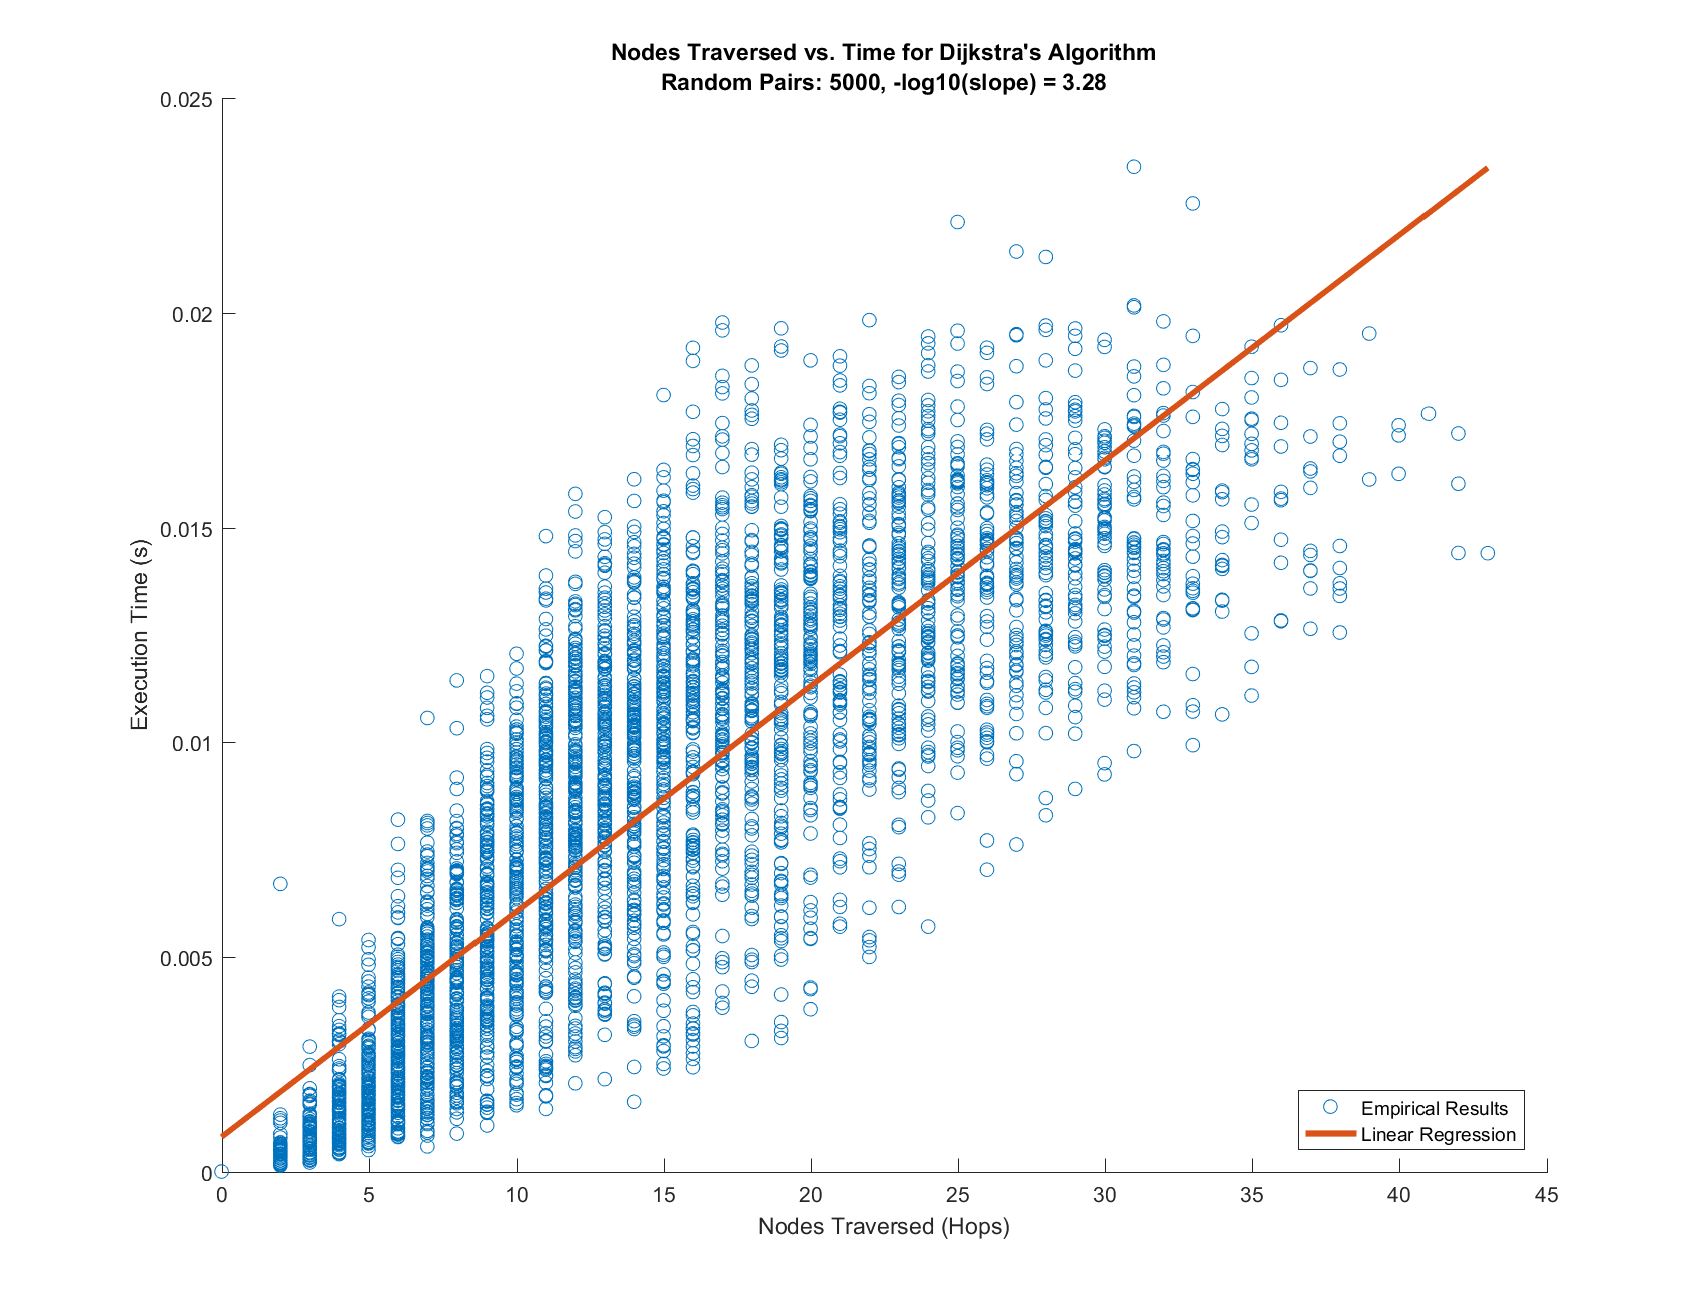
\includegraphics[width=0.8\textwidth]{dijkstraEmpirical}
\caption{Empirical results of Dijkstra's Algorithm.}
\end{figure}

Note that the theoretical time complexity is estimated by our linear regression, which has a slope of 3.28. The precise theoretical complexity is on the order of the number of vertices in the graph squared, \textit{i.e.} $O(|V|^2)$. There are 445 cities on our map, so the algorithm has a worst-case complexity of $O(445^2)$. This is a constant value as the big-O notation is simply a worst-case measure. As the algorithm stops early a majority of the time, it does not need to step through each node- especially if it is well connected as our map is.

\end{document}